\subsection*{Is it Time to Replace CNNs with Transformers for Medical Images?}

% \subsection*{Ссылка} \url{https://arxiv.org/abs/2108.09038}
\subsubsection*{Введение}
В течение последних лет сверточные нейронные сети (СНС)
являлись лидирующим методом в автоматической медицинской 
диагностике. Однако, недавно появившиеся vision transformers
(ViT) \cite{Transformers}, являются достойной альтернативной для СНС, достигая 
схожих уровней производительности, обладая некоторыми интересными свойствами,
которые могут быть полезными в задачах распознавания медицинских 
изображений. В данной работе исследуется возможность замены 
сверточных нейронных сетей трансформерами ViT в задачах 
медицинской автоматизации и какие плюсы это принесет. 
\subsubsection*{Основная идея}
Для того, чтобы получить ответ на поставленный вопрос, авторы работы \cite{ann11}
провели серию экспериментов, сравнивая ViT и СНС при одинаковых
условиях, минимально изменяя гиперпараметры. Чтобы обеспечить 
чистоту эксперимента, были выбраны ResNet50, как представитель СНС 
и DeiT-S, как представитель ViT, так как они сравнимы по 
количеству параметров, затратам памяти и вычислительным мощностям.
Инициализация СНС проводилась по трем стратегиям: (1) инициализация весов 
случайными значениями; (2) трансферное обучение (transfer learning) с 
с использованиям весов, предобученных на ImageNet; (3) self-supervised предобучение 
на целевом датасете, после инициализации как в пункте (2). Каждый эксперимент
повторялся пять раз и выбирались результаты с самой высокой точностью
на валидационном множестве.
\subsubsection*{Данные}
APTOS 2019, ISIC 2019, CBIS-DDSM
\subsubsection*{Результаты}
При случайной инициализации весов СНС превосходит ViT. Такая 
закономерность выявлена при обучении на всех трех датасетах.
Однако, при использовании весов, предобученных на ImageNet, 
разрыв между производительностью СНС и ViT в данной задаче 
сходит почти на нет.  Таким образом, можно заключить:
\begin{itemize}
    \item ViT проигрывает СНС при случайной инициализации 
    весов и обучении с нуля;
    \item Трансферное обучение устраняет разрыв в производительности
    между ViT и СНС;
    \item Наилучший результат получен при подходе self-supervised+
    pre-training+ fine-tuning, при котором ViT слегка превосходит СНС.
\end{itemize}


{\small
\begin{center}
    \footnotesize
    \captionof{table}{Сравнение результатов предсказания СНС и ViT в разрезе \\ различных стратегий инициализации весов 
    на медицинских изображениях.}
    \begin{tabular}{llccc}
    \toprule
    \textbf{Initialization} & \textbf{Model} & \textbf{APTOS2019}, $\kappa \uparrow$ & \textbf{ISIC2019}, Recall $\uparrow$ & \textbf{DDSM}, ROC-AUC $\uparrow$ 
    \\
    \midrule
    \multirow{2}{*}{Random}
    & ResNet50 & 0.849 $\pm$ 0.022 & 0.662 $\pm$ 0.018 & 0.917 $\pm$ 0.005 
    
    \\ 
    & DeiT-S   & 0.687 $\pm$ 0.017 & 0.579 $\pm$ 0.028 & 0.908 $\pm$ 0.015 
    
    \\[0.5em] %\hlineB{4} %\hline
    %%%%%%
    %%%%%%
    %%%%%%
    \multirow{2}{*}{ImageNet (supervised)} 
    & ResNet50 & 0.893 $\pm$ 0.004 & 0.810 $\pm$ 0.008 & 0.953 $\pm$ 0.008 
    
    \\ 
    & DeiT-S   & 0.896 $\pm$ 0.005 & 0.844 $\pm$ 0.021 & 0.947 $\pm$ 0.011 
    % & - $\pm$ - 
    \\[0.5em] %\hline
    %%%%%%
    %%%%%%
    %%%%%%
    \multirow{2}{*}{\begin{tabular}[c]{@{}l@{}}ImageNet (supervised) + \\ Self-supervised with DINO \end{tabular}} 
    & ResNet50 & 0.894 $\pm$ 0.008 & 0.833 $\pm$ 0.007 & 0.955 $\pm$ 0.002 
    % & - $\pm$ - 
    \\ 
    & DeiT-S   & 0.896 $\pm$ 0.010 & 0.853 $\pm$ 0.009 & 0.956 $\pm$ 0.002 
    % & - $\pm$ - 
    \\ 
    \bottomrule
    \end{tabular}
\end{center}
}

\begin{minipage}{1.0\linewidth}
    \begin{center}
        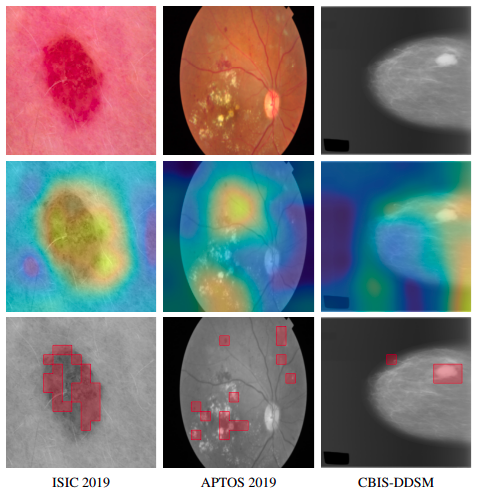
\includegraphics[scale=0.4]{ann11_res2.png} \\
        \captionof{figure}{\scriptsize{Сравнение карт значимости (saliency maps) изображений из трех датасетов. В каждой \\ 
        колонке представлены оригинальное изображение, визуализация ResNet50 Grad-CAM saliency map и карты \\ внимания (attention map) DEIT-S.}}
    \end{center}
    
\end{minipage}

\subsubsection*{Заключение}
В данной работе проводится анализ возможности замены сверточных
нейронных сетей трансформерами (ViT) в задачах распознавания
медицинских изображений. Показано, что ViT по качеству сравнима 
с СНС и может быть использована как альтернативный уже существующим метод.